% !TeX spellcheck = en_US
\documentclass[a4paper,12pt]{article}

\usepackage{fullpage}
\usepackage[utf8]{inputenc}
\usepackage{fourier}
\usepackage{amsmath}
\usepackage{color}
\usepackage{graphicx}
\usepackage{titlesec}
\usepackage{longtable}
\usepackage{wrapfig}

\titleformat{\section}[hang]{\Large\bfseries}{\Roman{section}\quad}{0pt}{}
\titleformat{\subsection}[hang]{\large\bfseries}{\arabic{subsection}.\quad}{0pt}{}
\titleformat{\subsubsection}[hang]{\large}{\arabic{subsection}\alph{subsubsection})\quad}{0pt}{}

\newcommand{\twodo}[1]{\textcolor{red}{\textbf{todo:} #1}}

\title{\textbf{Exercises for Image Processing 1}\\Problem Sheet 5}
\author{Tim Dobert\\6427948 \and Konstantin M\"ollers\\6313136}

\begin{document}
	\maketitle	
	
	\section{Theoretical Problems}
	\subsection{(Lossless) Image Compression}
	
	\subsubsection{Entropy}
	
	We calculate the entropy of the document by obtaining the mean number of bits which are required to encode the information of this source. Therefor, we are determine the mean value of all expectable number of bits needed to encode each value. The mean of a value array is calculated by a weighted sum of those values; with the probability being the weight.
	
	\begin{align*}
	\text{Num. of values }G	&= 6 \\
	\text{Entropy } H 	&= \sum\limits_{g = 0}^{G - 1} P(g) \cdot \log_2 \frac{1}{P(g)} 	\\
		&\approx 0.136803+ 0.291508+ 0.0382193+ 0.00996578+ 0.0179316+ 0.0765699\\
		&= 0.570998
	\end{align*}
	
	\subsubsection{Huffman Code}
	
	First of all, we calculate the actual probabilities for the classification in combination with their colors. Because of the independence of these values, we can obtain those just by multiplication.
	
	\begin{table}[h!]
		\centering
		\begin{tabular}{l|l|l|r|l|r}
			$g$ & \textbf{Classification} & \textbf{Color} & \textbf{Probability} $P(g)$ & \textbf{Huffman Code} & \textbf{Length} $l(g)$ \\\hline
			0 & background & white & 0.900 & \texttt{0} & 1 \\
			1 & print & black & 0.080 & \texttt{10} & 2 \\
			2 & print & red & 0.005 & \texttt{1110} & 4\\
			3 & print & yellow & 0.001 & \texttt{11111} & 5\\
			4 & print & green & 0.002 & \texttt{11110} & 5\\
			5 & print & blue & 0.012 & \texttt{110} & 3\\\hline
			\multicolumn{3}{l|}{$\Sigma$} & 1.000 & \multicolumn{2}{r}{1.131}
		\end{tabular}
	\end{table}
	
	The Huffman code gets calculated by giving the smallest probabilities a binary code (either \texttt{0} or \texttt{1}) and summing up their probabilities. We then compare the sum with other values and iterate. In the end, you get a code The way we calculated the Huffman code is presented in the following schema.
	
	\begin{figure}[h!]
		\centering
		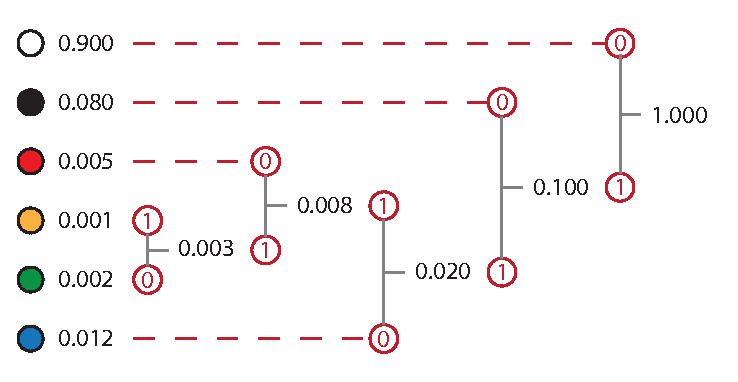
\includegraphics[width=0.7\textwidth]{huffman.pdf}
	\end{figure}
	
	\newpage
	
	\subsubsection{Mean Length}
	
	To calculate the mean length $b_\text{Huffman}$ of our Huffman code, we just need to sum up the probability-weighted code lengths of all pixel values.
	
	\begin{align*}
		b_\text{Huffman} &= \sum\limits_{g = 0}^{G - 1} P(g) \cdot l(g)\\
			&= 0.900 \cdot 1\\
			&+ 0.080 \cdot 2\\
			&+ 0.005 \cdot 4\\
			&+ 0.001 \cdot 5\\
			&+ 0.002 \cdot 5\\
			&+ 0.012 \cdot 3 = 1.131
	\end{align*}
	
	{\footnotesize Redundancy $r_\text{Huffman} = 1.131 - 0.570998 = 0.560002$.}
	
	\subsubsection{Redundancy}
	
	{\footnotesize With formulas from Lecture 08, Slide 5:}
	\begin{align*}
		\text{Num. bits per pixel }b_\text{4-bit} &= 4 \\
		\text{Entropy }H &\approx 0.570998\\
		\text{Redundancy }r_\text{4-bit} &= b_\text{4-bit} - H \approx 3.429002
	\end{align*}
	
	
	\noindent As we can see, our Huffman code is much less redundant than the 4-bit code given from the exercise; as the latter has a redundancy value of 3.429002 whether the former has just one of 0.560002.
	
	\subsection{Image Segmentation}
	\subsubsection{}
	Thresholding only works if the brightness values of the segments are different from the background. They also need to be consistent within the segment. It would work well for black text on white background photographed with even lighting. If the lighting is in inconsistent and the letters have gradient colors or other patterns, it might lead to wrong results.
	\begin{figure}[h]
	\center
	\fbox{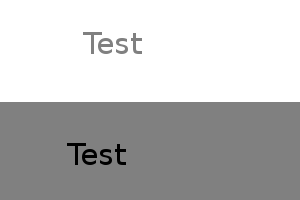
\includegraphics[scale=0.5]{threshold_ex.png}}\\
	\caption{Another example for when thresholding does not work for segmentation.}
	\end{figure}
	
	\subsubsection{}
	The Bimodality does not guarantee a successful segmentation by thresholding. If there are multiple light sources, the contrast along an edge can be reversed. As an example, consider the picture of the Michaelis Church from the lecture. Its histogram is bimodal but thresholding would not be able to segment correctly along the vertical edge.
	
	\subsubsection{}	
	Component labeling is necessary to identify connected areas correctly.
	
	\subsubsection{}
	The most typical problem in edge detection is separating real edges from noise. If the edge detection is too sensitive, it will falsely identify noise as edges, if it is not sensitive enough it will miss actual edges. The Canny Operator aims to solve this problem by convolving the image with Gaussian filters of different scales and compiling the results using feature synthesis. 
	
	\section{Practical Problems}
	\subsection{(Lossy) Image Compression}
	\subsubsection{Matrix}
	$A_3 =
	\begin{pmatrix}
	0.5 & 0.5 & 0.5 & 0.5\\
	0.5 & -0.5 & 0.5 & -0.5\\
	-0.5 & -0.5 & 0.5 & 0.5\\
    \end{pmatrix}		
	$
	\subsubsection{Error}
	$MSE = 2.5175756233 \cdot 10^{-30}$
	
	\newlength{\colwidth}
	\newlength{\colsep}
	\setlength{\colsep}{8mm}
	\setlength{\colwidth}{\dimexpr.25\textwidth-.75\colsep}
	
	\begin{wrapfigure}{r}{\colwidth}
		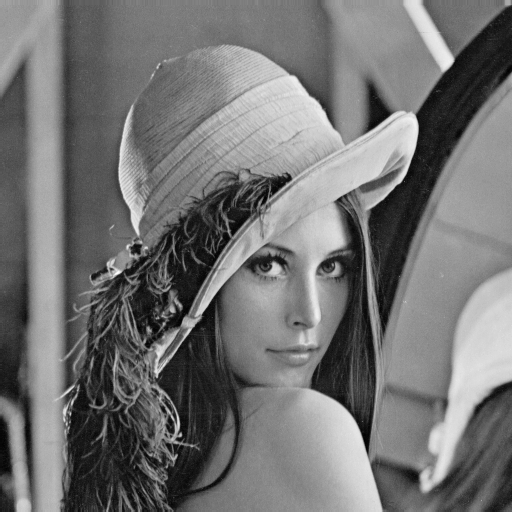
\includegraphics[width=\colwidth]{lena}
		
		Original Image
	\end{wrapfigure}
	
	\subsection{Operators for Edge detection}
	
	The Kirsch, Sobel and Scharr operators are not as susceptible to noise as the other two and are thus preferable in real world scenarios. We would prefer the \textbf{Sobel operator} most, because with it it's the easiest to recognize details of the face like eyes, lips and nose.
	
	This how the angles are colored in the following direction images: \quad
	
%		
		\subsubsection{Robert's Cross operator}
		Looks very noisy
		
		\begin{longtable}{@{}p{\colwidth}@{\hspace*{\colsep}}p{\colwidth}@{\hspace{\colsep}}p{\colwidth}@{\hspace{\colsep}}p{\colwidth}@{}}
			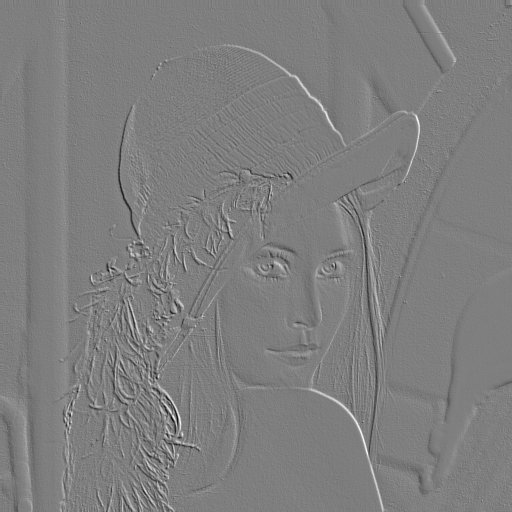
\includegraphics[width=\linewidth]{img/roberts_cross_real} &
			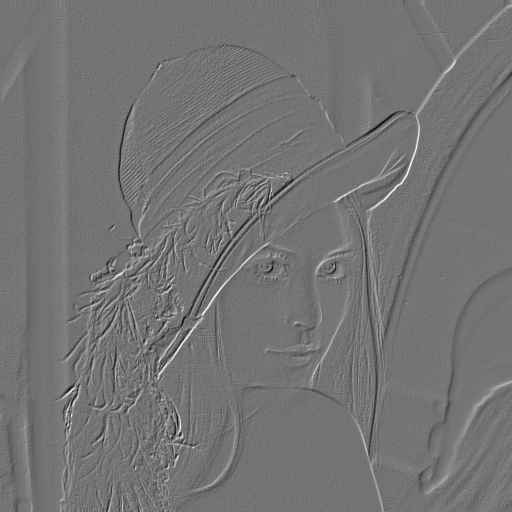
\includegraphics[width=\linewidth]{img/roberts_cross_imag} &
			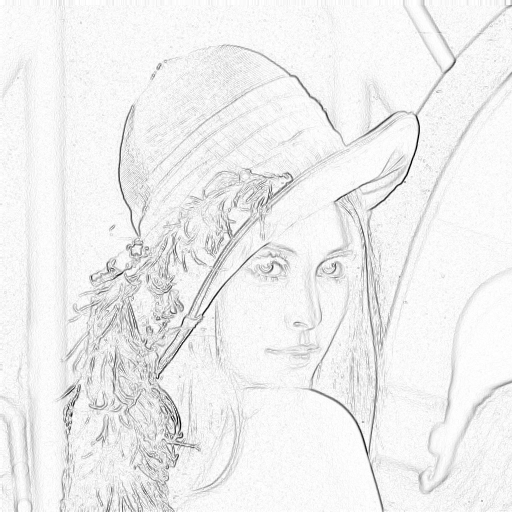
\includegraphics[width=\linewidth]{img/roberts_cross_magnitudes} &
			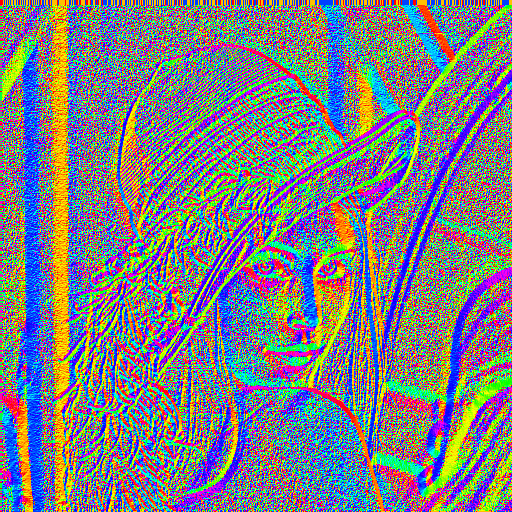
\includegraphics[width=\linewidth]{img/roberts_cross_directions} \\
			Diagonal top right to bottom left &
			Diagonal bottom right to top left &
			Magnitudes $|\nabla g|$ &
			Directions \\
		\end{longtable}
%		
		\subsubsection{Sobel operator}
		\begin{longtable}{@{}p{\colwidth}@{\hspace*{\colsep}}p{\colwidth}@{\hspace{\colsep}}p{\colwidth}@{\hspace{\colsep}}p{\colwidth}@{}}
			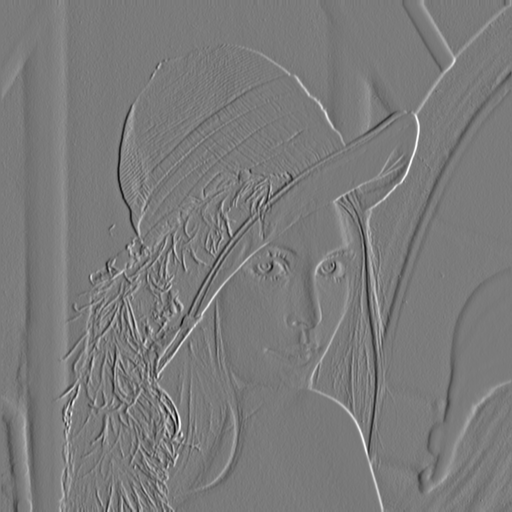
\includegraphics[width=\linewidth]{img/sobel_real} &
			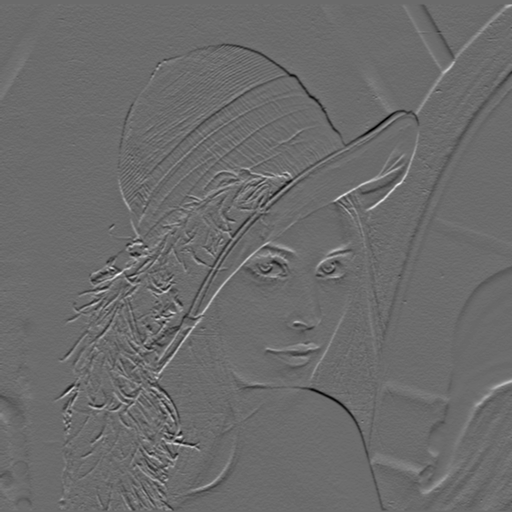
\includegraphics[width=\linewidth]{img/sobel_imag} &
			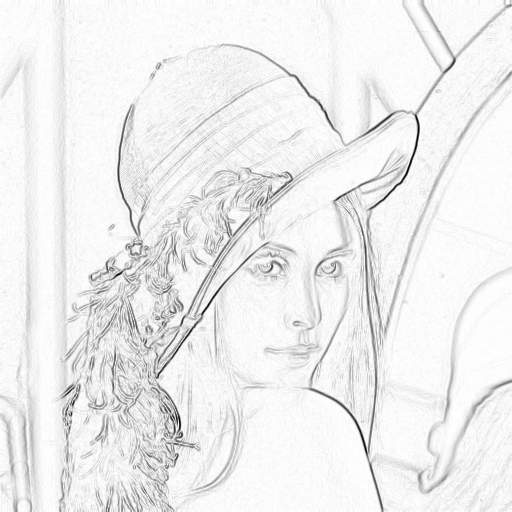
\includegraphics[width=\linewidth]{img/sobel_magnitudes} &
			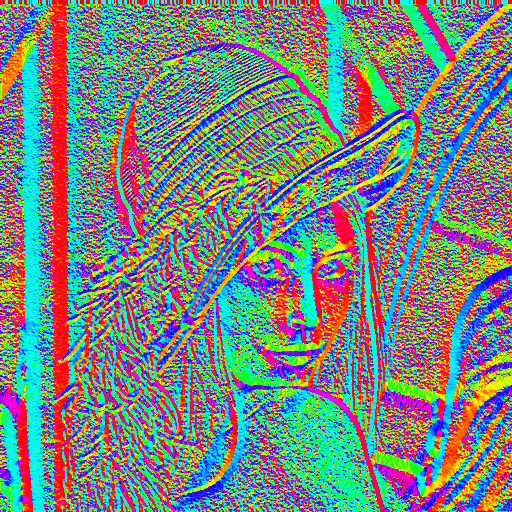
\includegraphics[width=\linewidth]{img/sobel_directions} \\
			X-Deviation $\frac{\partial x}{\partial g}$ &
			Y-Deviation $\frac{\partial y}{\partial g}$ &
			Magnitudes $|\nabla g|$ &
			Directions \\
		\end{longtable}
		
		\subsubsection{Kirsch operator}
		\begin{longtable}{@{}p{\colwidth}@{\hspace*{\colsep}}p{\colwidth}@{\hspace{\colsep}}p{\colwidth}@{\hspace{\colsep}}p{\colwidth}@{}}
%			\includegraphics[width=\linewidth]{img/kirsch_real} &
%			\includegraphics[width=\linewidth]{img/kirsch_imag} &
			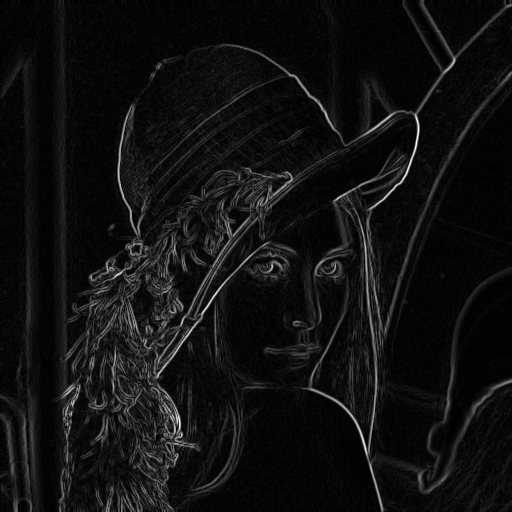
\includegraphics[width=\linewidth]{img/kirsch_magnitudes} &
			\includegraphics[width=\linewidth]{img/kirsch_directions} &&\\
%			X-Deviation $\frac{\partial x}{\partial g}$ &
%			Y-Deviation $\frac{\partial y}{\partial g}$ &
			Magnitudes $|\nabla g|$ &
			Directions &&\\
		\end{longtable}
%		& \raisebox{-\totalheight}{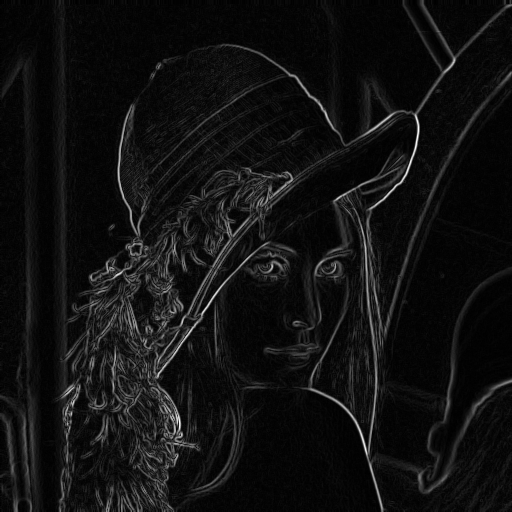
\includegraphics[width=\linewidth]{kirsch_magnitudes}} \linebreak \textit{Magnitudes}
%		& \raisebox{-\totalheight}{\includegraphics[width=\linewidth]{kirsch_directions}} \linebreak \textit{Directions}\\
%%		
		\subsubsection{Laplacian operator}
		\begin{longtable}{@{}p{\colwidth}@{\hspace*{\colsep}}p{\colwidth}@{\hspace{\colsep}}p{\colwidth}@{\hspace{\colsep}}p{\colwidth}@{}}
			%			\includegraphics[width=\linewidth]{kirsch_real} &
			%			\includegraphics[width=\linewidth]{kirsch_imag} &
			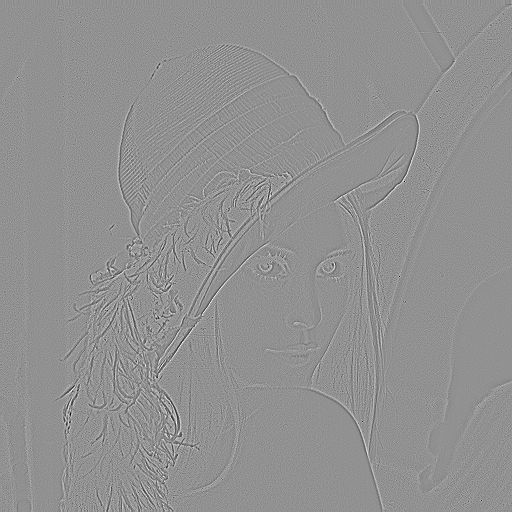
\includegraphics[width=\linewidth]{img/laplacian_real} &&&\\
%			\includegraphics[width=\linewidth]{kirsch_directions} &&\\
			%			X-Deviation $\frac{\partial x}{\partial g}$ &
			%			Y-Deviation $\frac{\partial y}{\partial g}$ &
			Derivative $\nabla^2 g$ &&&\\
%			Directions &&\\
		\end{longtable}

		\subsubsection{Extra: Scharr operator}
		\begin{longtable}{@{}p{\colwidth}@{\hspace*{\colsep}}p{\colwidth}@{\hspace{\colsep}}p{\colwidth}@{\hspace{\colsep}}p{\colwidth}@{}}
			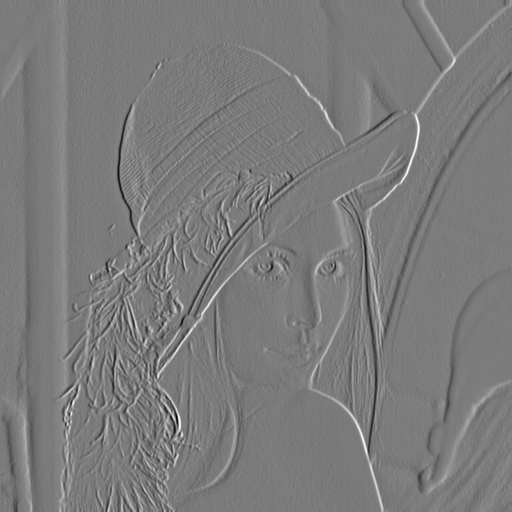
\includegraphics[width=\linewidth]{img/scharr_real} &
			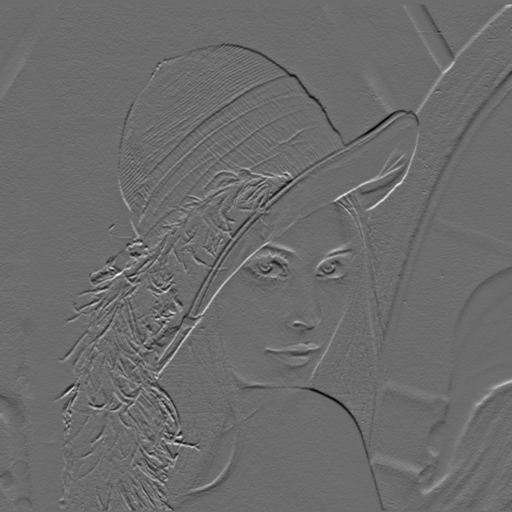
\includegraphics[width=\linewidth]{img/scharr_imag} &
			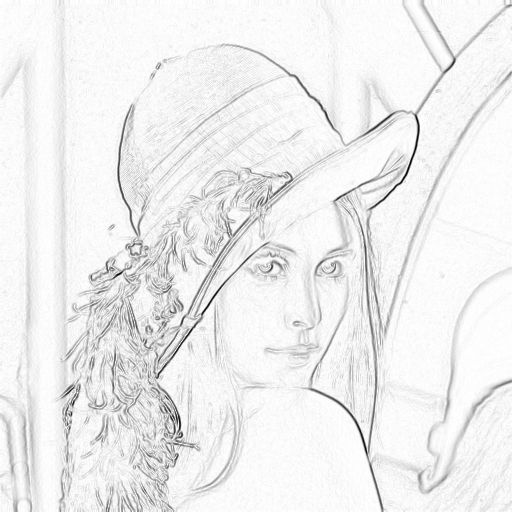
\includegraphics[width=\linewidth]{img/scharr_magnitudes} &
			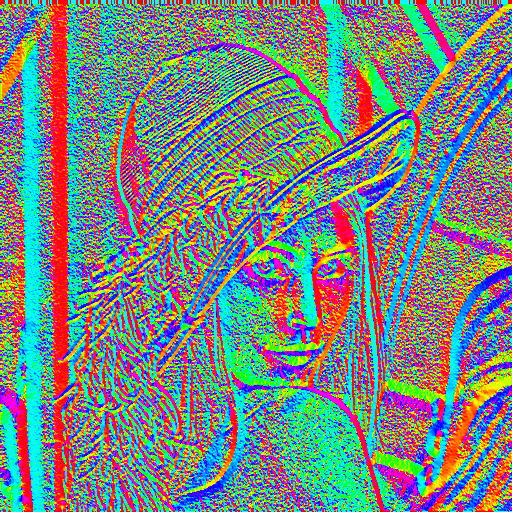
\includegraphics[width=\linewidth]{img/scharr_directions} \\
			X-Deviation $\frac{\partial x}{\partial g}$ &
			Y-Deviation $\frac{\partial y}{\partial g}$ &
			Magnitudes $|\nabla g|$ &
			Directions \\
		\end{longtable}
\end{document}
